\chapter{Question 3}
\label{available-representation}

\textbf{Cluster the blogs using K-Means, using k=5,10,20. (see slide 18).  Print the values in each centroid, for each value of k.  How many interations were required for each value of k?}\\\\

Following are the steps I have taken to solve the problem:
\begin{itemize}
\item I imported the `clusters.py' mentioned in `question 2' and used the code described in `presentation slide 18' to cluster the blogs using K-Means, using k= 5, 10, 20. The output prints the values in each centroid, for each value of k and also the number of iterations required for each value of k. This code is in Listing \ref{lst:q3code1} 
\newpage
\item The output file is uploaded to github at \url{https://github.com/majetisiri/cs532-s16/blob/master/a8/q3-numberOfIterationsAndValuesInEachCentroid.txt}. The sample output is illustrated in Figure \ref{fig:q3fig1}. 
\begin{figure}[h!]
\begin{center}
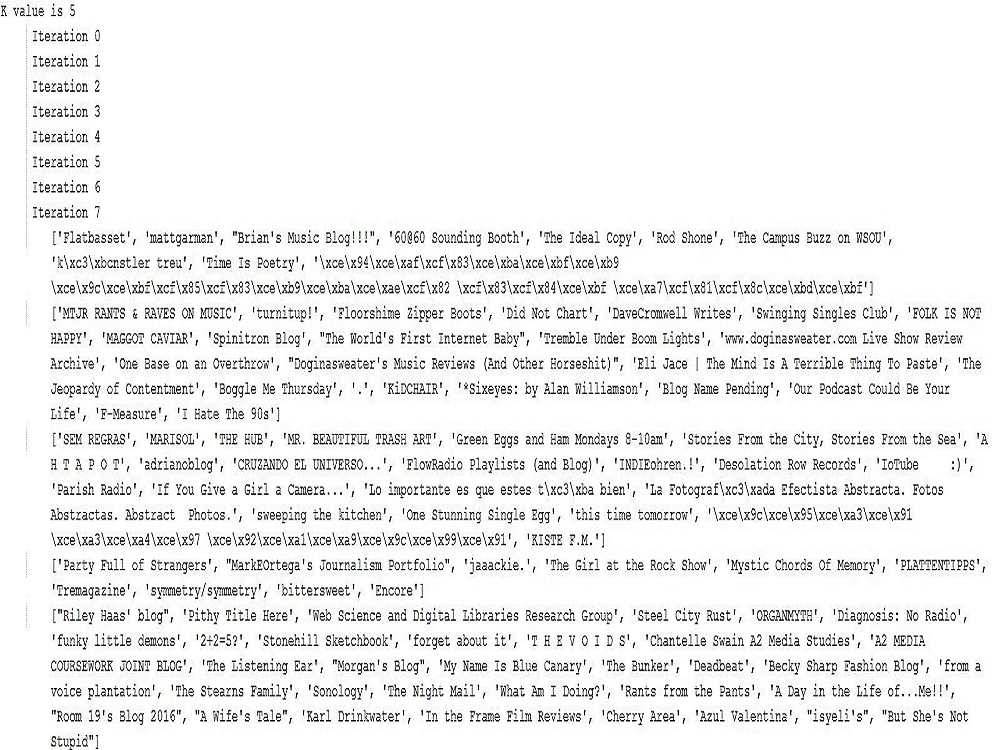
\includegraphics[scale=0.55, keepaspectratio=true]{figures/3.JPG}
\caption{Sample output with number of iterations and values in each centroid for k=5}
\label{fig:q3fig1}
\end{center}
\end{figure}
\end{itemize}


\newpage
\textbf{Code Listing}
\sloppy
\lstinputlisting[language=Python,caption=Python code for generating ASCII,frame=single,breaklines=true,label=lst:q3code1, tabsize=2, captionpos=b,numbers=left,showspaces=false,showstringspaces=false,basicstyle=\footnotesize]{src/getKmeans.py}

